As noted during the disscussion of the design of the system the front end of the system is respobsible for the processing
the input from the user and relaying the data produced by the back-end back to the user.

As this stage is primeraly responsible
for performing input output operations it is unlikely to end up being a bottleneck in the operation of the syste, as a
result the implementation has not been optimised to perform its role as efficiently as possible to allow more resources
to be allocated to the development of the back-end.

\subsection{Scene Input}
Scene input begins by reading from a file pointed to by the user and if not given a default file defined in the source
code, this file is a list of all objects in the scene (see Appendix~\ref{chap:scene-appendix} for a full descritption.) each
object described is created and stored in structure (see Figure~\ref{fig:scene_define}) each of the objects in the
file may be completly specified from the scene file such as lights and cameras while other objects such as meshes
and spheres may require other files to be read containing data such as material properties and vertex information.

\subsubsection{Mesh Input}
If a mesh is specified in the scene file the vertex information will be read from a ply file, this data is just a list
of vertices, normals texture coordinated and triangle indices, this structure is not conducive to efficient intersection
tests, as a result a k-d tree is created before storing the mesh in the scene, k-d tree construction will be discussed in
Section~\ref{sec:obj_mesh}

\subsection{Command Line}
Users are able to input command line arguments to the system, these are received by C programs in the input parameters of
the main function, these input parameters need to be parsed and stored, this is performed by simply scanning over each
option in the argv list to find a valid option or pair of options in the case of a user inputed value for the option
i.e. width of the output image.

\begin{figure}[h]
\texttt{./raytracer -w 1000 -h 1000 -i ./data/scenes/cornell\_box.scene}
\caption{Example command line.}
\end{figure}

\subsection{Global Configuration}
Once the configuration of the scene has been read and processed the data containing the configuration will not change for
the lifetime of the program, as a result the global configuration is available in the system through a global variable, while
it is generally advised whene developing software that global variable should be avoided an implementation that passed the
configuration would require that a pointer to a configuration structure be passed, this amounts to having the same result
as a global variable whilst reducing the clarity of the code, although we do lose the ability to specify a const qualifier
to prevent modification and as a result care had to be taken that no variable in the configuration structure was modified.

\begin{figure}
\centering
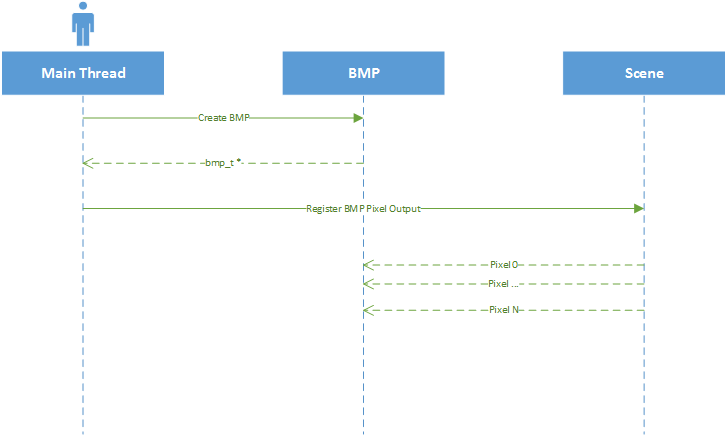
\includegraphics[width=\textwidth]{./images/pixel_update_sequence.png}
\caption{Sequence for pixel update}
\end{figure}

\subsection{Common Pixel Update Interface}
As part of the decoupling of the input/output of the system and the image synthesis we have decided to create an interface
between the fron and back-end that will be used to send pixel data to the front end, this interface allows for a callback to
be registered that will be called for each of the pixels in the output image, multiple callbacks can be registered allowing
for the interface to be used for multiple purporses, Two modules have been created that use the interface to demonstrate the
useage of the interface, these are described below.

\subsubsection{Image Output}

The systems output default image format is BMP, this image format was chosen as it is a simple image format, there are
several variants of BMP each with its own header definition the version of BMP that is implemented is the OS/2 bitmap this is
one of the more simple variants with a fixed size header that specified few options. The implementation of the BMP output can
be found in \texttt{bmp.h/c}. If supported on the platform the system is also capable of outputing images in PNG file format,
this is acheived by using libPNG, there are advantages to outputing to this format, foremost is that the image size of an
image output to PNG is significantally smaller than that outputed by BMP.

\subsubsection{GUI}

The user interface that is included in the system is designed to allow instant feedback to the user of the render, this can be
useful in the case of errors that can be identified early in what may be a costly render, the interface is rather simple
providing a surface that displays the current state of the render.

We have decided to use SDL library to provide the interface to the operating system window system and OpenGL to perform the 
drawing of the pixels to the screen. SDL (Simple Direct media Library) is a library that allows for cross platform applications to be written that include
drawable surfaces, OpenGL support and user input, SDL is written in C and provides a library API for C.

The surface that the image is displayed on is implemented as a OpenGL textured quad that spans the width and height of the screen.
The callback function that is defined for the GUI writes each pixel value to a queue which will be read by the render mainloop,
this mainloop will read the pixel data and update the appropreate location in the texture with that value, in order to reduce the
number of draw calls made by the GUI multiple pixels can be updated before each draw call, this is implemented by performing
a non blocking read until we cannot read any pixels without blocking, we will then perform the draw call.

In order to retain responsivness of the GUI while rendering it is desirable to run the GUI on a seperate thread, the GUI
should also only redraw the screen when a pixel has updated its colour, this is to reduce the amount of processing that
the GUI is performing that could be used to create images, on the other had the GUI should respond to events that are pushed
to its internal event queue such as key presses and window system events, Figure~\ref{fig:gui_screenshot} demonstrates the
gui running.

\begin{figure}[h]
\centering
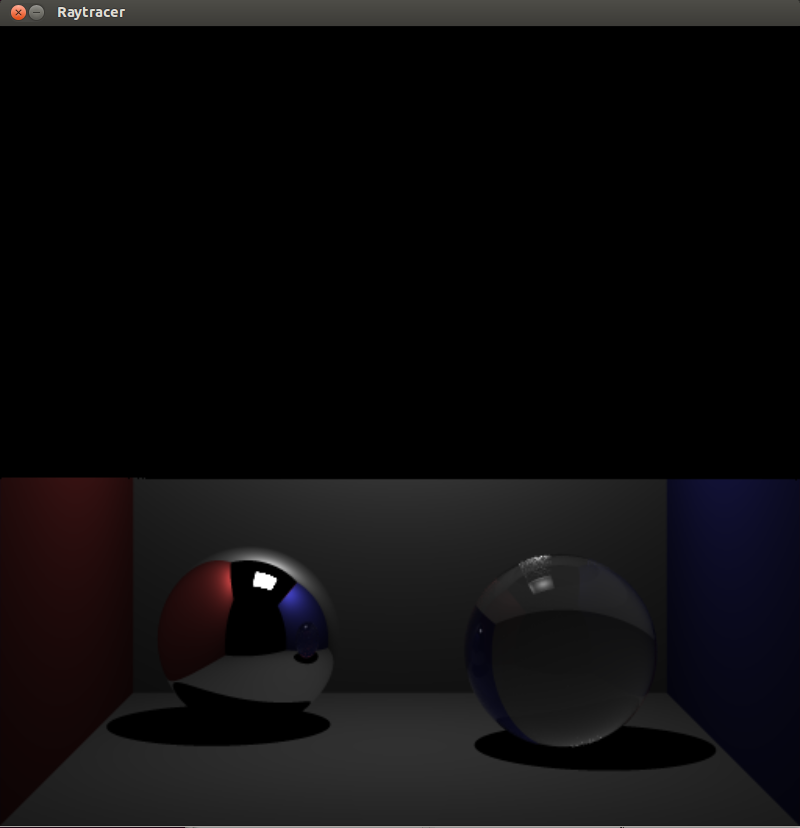
\includegraphics[scale=0.24]{./images/gui_screenshot.png}
\caption{Screenshot of render in progress}
\label{fig:gui_screenshot}
\end{figure}
